% Options for packages loaded elsewhere
\PassOptionsToPackage{unicode}{hyperref}
\PassOptionsToPackage{hyphens}{url}
%
\documentclass[
]{book}
\usepackage{lmodern}
\usepackage{amssymb,amsmath}
\usepackage{ifxetex,ifluatex}
\ifnum 0\ifxetex 1\fi\ifluatex 1\fi=0 % if pdftex
  \usepackage[T1]{fontenc}
  \usepackage[utf8]{inputenc}
  \usepackage{textcomp} % provide euro and other symbols
\else % if luatex or xetex
  \usepackage{unicode-math}
  \defaultfontfeatures{Scale=MatchLowercase}
  \defaultfontfeatures[\rmfamily]{Ligatures=TeX,Scale=1}
\fi
% Use upquote if available, for straight quotes in verbatim environments
\IfFileExists{upquote.sty}{\usepackage{upquote}}{}
\IfFileExists{microtype.sty}{% use microtype if available
  \usepackage[]{microtype}
  \UseMicrotypeSet[protrusion]{basicmath} % disable protrusion for tt fonts
}{}
\makeatletter
\@ifundefined{KOMAClassName}{% if non-KOMA class
  \IfFileExists{parskip.sty}{%
    \usepackage{parskip}
  }{% else
    \setlength{\parindent}{0pt}
    \setlength{\parskip}{6pt plus 2pt minus 1pt}}
}{% if KOMA class
  \KOMAoptions{parskip=half}}
\makeatother
\usepackage{xcolor}
\IfFileExists{xurl.sty}{\usepackage{xurl}}{} % add URL line breaks if available
\IfFileExists{bookmark.sty}{\usepackage{bookmark}}{\usepackage{hyperref}}
\hypersetup{
  pdftitle={The statistics reference book for judges},
  pdfauthor={Harry Gray},
  hidelinks,
  pdfcreator={LaTeX via pandoc}}
\urlstyle{same} % disable monospaced font for URLs
\usepackage{color}
\usepackage{fancyvrb}
\newcommand{\VerbBar}{|}
\newcommand{\VERB}{\Verb[commandchars=\\\{\}]}
\DefineVerbatimEnvironment{Highlighting}{Verbatim}{commandchars=\\\{\}}
% Add ',fontsize=\small' for more characters per line
\usepackage{framed}
\definecolor{shadecolor}{RGB}{248,248,248}
\newenvironment{Shaded}{\begin{snugshade}}{\end{snugshade}}
\newcommand{\AlertTok}[1]{\textcolor[rgb]{0.94,0.16,0.16}{#1}}
\newcommand{\AnnotationTok}[1]{\textcolor[rgb]{0.56,0.35,0.01}{\textbf{\textit{#1}}}}
\newcommand{\AttributeTok}[1]{\textcolor[rgb]{0.77,0.63,0.00}{#1}}
\newcommand{\BaseNTok}[1]{\textcolor[rgb]{0.00,0.00,0.81}{#1}}
\newcommand{\BuiltInTok}[1]{#1}
\newcommand{\CharTok}[1]{\textcolor[rgb]{0.31,0.60,0.02}{#1}}
\newcommand{\CommentTok}[1]{\textcolor[rgb]{0.56,0.35,0.01}{\textit{#1}}}
\newcommand{\CommentVarTok}[1]{\textcolor[rgb]{0.56,0.35,0.01}{\textbf{\textit{#1}}}}
\newcommand{\ConstantTok}[1]{\textcolor[rgb]{0.00,0.00,0.00}{#1}}
\newcommand{\ControlFlowTok}[1]{\textcolor[rgb]{0.13,0.29,0.53}{\textbf{#1}}}
\newcommand{\DataTypeTok}[1]{\textcolor[rgb]{0.13,0.29,0.53}{#1}}
\newcommand{\DecValTok}[1]{\textcolor[rgb]{0.00,0.00,0.81}{#1}}
\newcommand{\DocumentationTok}[1]{\textcolor[rgb]{0.56,0.35,0.01}{\textbf{\textit{#1}}}}
\newcommand{\ErrorTok}[1]{\textcolor[rgb]{0.64,0.00,0.00}{\textbf{#1}}}
\newcommand{\ExtensionTok}[1]{#1}
\newcommand{\FloatTok}[1]{\textcolor[rgb]{0.00,0.00,0.81}{#1}}
\newcommand{\FunctionTok}[1]{\textcolor[rgb]{0.00,0.00,0.00}{#1}}
\newcommand{\ImportTok}[1]{#1}
\newcommand{\InformationTok}[1]{\textcolor[rgb]{0.56,0.35,0.01}{\textbf{\textit{#1}}}}
\newcommand{\KeywordTok}[1]{\textcolor[rgb]{0.13,0.29,0.53}{\textbf{#1}}}
\newcommand{\NormalTok}[1]{#1}
\newcommand{\OperatorTok}[1]{\textcolor[rgb]{0.81,0.36,0.00}{\textbf{#1}}}
\newcommand{\OtherTok}[1]{\textcolor[rgb]{0.56,0.35,0.01}{#1}}
\newcommand{\PreprocessorTok}[1]{\textcolor[rgb]{0.56,0.35,0.01}{\textit{#1}}}
\newcommand{\RegionMarkerTok}[1]{#1}
\newcommand{\SpecialCharTok}[1]{\textcolor[rgb]{0.00,0.00,0.00}{#1}}
\newcommand{\SpecialStringTok}[1]{\textcolor[rgb]{0.31,0.60,0.02}{#1}}
\newcommand{\StringTok}[1]{\textcolor[rgb]{0.31,0.60,0.02}{#1}}
\newcommand{\VariableTok}[1]{\textcolor[rgb]{0.00,0.00,0.00}{#1}}
\newcommand{\VerbatimStringTok}[1]{\textcolor[rgb]{0.31,0.60,0.02}{#1}}
\newcommand{\WarningTok}[1]{\textcolor[rgb]{0.56,0.35,0.01}{\textbf{\textit{#1}}}}
\usepackage{longtable,booktabs}
% Correct order of tables after \paragraph or \subparagraph
\usepackage{etoolbox}
\makeatletter
\patchcmd\longtable{\par}{\if@noskipsec\mbox{}\fi\par}{}{}
\makeatother
% Allow footnotes in longtable head/foot
\IfFileExists{footnotehyper.sty}{\usepackage{footnotehyper}}{\usepackage{footnote}}
\makesavenoteenv{longtable}
\usepackage{graphicx,grffile}
\makeatletter
\def\maxwidth{\ifdim\Gin@nat@width>\linewidth\linewidth\else\Gin@nat@width\fi}
\def\maxheight{\ifdim\Gin@nat@height>\textheight\textheight\else\Gin@nat@height\fi}
\makeatother
% Scale images if necessary, so that they will not overflow the page
% margins by default, and it is still possible to overwrite the defaults
% using explicit options in \includegraphics[width, height, ...]{}
\setkeys{Gin}{width=\maxwidth,height=\maxheight,keepaspectratio}
% Set default figure placement to htbp
\makeatletter
\def\fps@figure{htbp}
\makeatother
\setlength{\emergencystretch}{3em} % prevent overfull lines
\providecommand{\tightlist}{%
  \setlength{\itemsep}{0pt}\setlength{\parskip}{0pt}}
\setcounter{secnumdepth}{5}
\usepackage{booktabs}
\usepackage{booktabs}
\usepackage{longtable}
\usepackage{array}
\usepackage{multirow}
\usepackage{wrapfig}
\usepackage{float}
\usepackage{colortbl}
\usepackage{pdflscape}
\usepackage{tabu}
\usepackage{threeparttable}
\usepackage{threeparttablex}
\usepackage[normalem]{ulem}
\usepackage{makecell}
\usepackage{xcolor}
\usepackage[]{natbib}
\bibliographystyle{apalike}

\title{The statistics reference book for judges}
\author{Harry Gray}
\date{2020-05-05}

\begin{document}
\maketitle

{
\setcounter{tocdepth}{1}
\tableofcontents
}
\hypertarget{preface}{%
\chapter*{Preface}\label{preface}}
\addcontentsline{toc}{chapter}{Preface}

This section will contain information about the book.

\hypertarget{what-does-this-book-contain}{%
\section*{What does this book contain?}\label{what-does-this-book-contain}}
\addcontentsline{toc}{section}{What does this book contain?}

\hypertarget{when-should-it-be-used}{%
\section*{When should it be used?}\label{when-should-it-be-used}}
\addcontentsline{toc}{section}{When should it be used?}

\hypertarget{intro}{%
\chapter{Introduction}\label{intro}}

You can label chapter and section titles using \texttt{\{\#label\}} after them, e.g., we can reference Chapter \ref{intro}. If you do not manually label them, there will be automatic labels anyway, e.g., Chapter \ref{false-positives}.

Figures and tables with captions will be placed in \texttt{figure} and \texttt{table} environments, respectively.

\begin{Shaded}
\begin{Highlighting}[]
\KeywordTok{par}\NormalTok{(}\DataTypeTok{mar =} \KeywordTok{c}\NormalTok{(}\DecValTok{4}\NormalTok{, }\DecValTok{4}\NormalTok{, }\FloatTok{.1}\NormalTok{, }\FloatTok{.1}\NormalTok{))}
\KeywordTok{plot}\NormalTok{(pressure, }\DataTypeTok{type =} \StringTok{'b'}\NormalTok{, }\DataTypeTok{pch =} \DecValTok{19}\NormalTok{)}
\end{Highlighting}
\end{Shaded}

\begin{figure}

{\centering 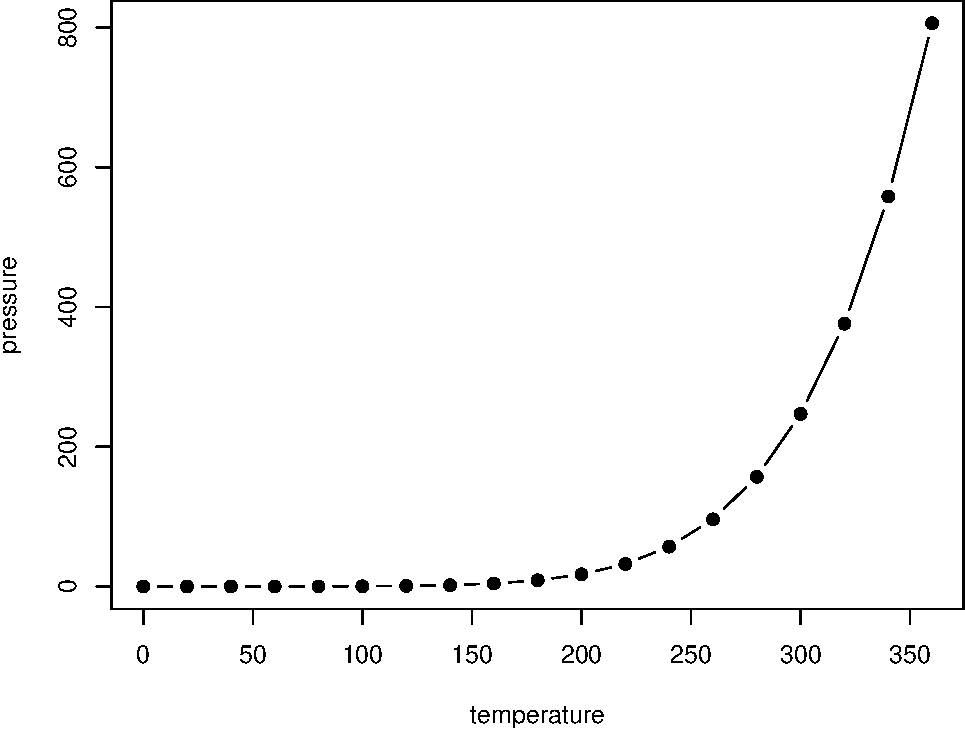
\includegraphics[width=0.8\linewidth]{01-intro_files/figure-latex/nice-fig-1} 

}

\caption{Here is a nice figure!}\label{fig:nice-fig}
\end{figure}

Reference a figure by its code chunk label with the \texttt{fig:} prefix, e.g., see Figure \ref{fig:nice-fig}. Similarly, you can reference tables generated from \texttt{knitr::kable()}, e.g., see Table \ref{tab:nice-tab}.

\begin{Shaded}
\begin{Highlighting}[]
\NormalTok{knitr}\OperatorTok{::}\KeywordTok{kable}\NormalTok{(}
  \KeywordTok{head}\NormalTok{(iris, }\DecValTok{20}\NormalTok{), }\DataTypeTok{caption =} \StringTok{'Here is a nice table!'}\NormalTok{,}
  \DataTypeTok{booktabs =} \OtherTok{TRUE}
\NormalTok{)}
\end{Highlighting}
\end{Shaded}

\begin{table}

\caption{\label{tab:nice-tab}Here is a nice table!}
\centering
\begin{tabular}[t]{rrrrl}
\toprule
Sepal.Length & Sepal.Width & Petal.Length & Petal.Width & Species\\
\midrule
5.1 & 3.5 & 1.4 & 0.2 & setosa\\
4.9 & 3.0 & 1.4 & 0.2 & setosa\\
4.7 & 3.2 & 1.3 & 0.2 & setosa\\
4.6 & 3.1 & 1.5 & 0.2 & setosa\\
5.0 & 3.6 & 1.4 & 0.2 & setosa\\
\addlinespace
5.4 & 3.9 & 1.7 & 0.4 & setosa\\
4.6 & 3.4 & 1.4 & 0.3 & setosa\\
5.0 & 3.4 & 1.5 & 0.2 & setosa\\
4.4 & 2.9 & 1.4 & 0.2 & setosa\\
4.9 & 3.1 & 1.5 & 0.1 & setosa\\
\addlinespace
5.4 & 3.7 & 1.5 & 0.2 & setosa\\
4.8 & 3.4 & 1.6 & 0.2 & setosa\\
4.8 & 3.0 & 1.4 & 0.1 & setosa\\
4.3 & 3.0 & 1.1 & 0.1 & setosa\\
5.8 & 4.0 & 1.2 & 0.2 & setosa\\
\addlinespace
5.7 & 4.4 & 1.5 & 0.4 & setosa\\
5.4 & 3.9 & 1.3 & 0.4 & setosa\\
5.1 & 3.5 & 1.4 & 0.3 & setosa\\
5.7 & 3.8 & 1.7 & 0.3 & setosa\\
5.1 & 3.8 & 1.5 & 0.3 & setosa\\
\bottomrule
\end{tabular}
\end{table}

You can write citations, too. For example, we are using the \textbf{bookdown} package \citep{R-bookdown} in this sample book, which was built on top of R Markdown and \textbf{knitr} \citep{xie2015}.

\hypertarget{uncertainty}{%
\chapter{Uncertainty}\label{uncertainty}}

This Chapter will be about uncertainty, probability, and statistics.

\hypertarget{false-positives}{%
\chapter{False positives and false negatives}\label{false-positives}}


\includegraphics{03-false-positives_files/figure-latex/title-image-1.pdf}

This Chapter introduces false positives and false negatives.

\hypertarget{what-are-false-positives-and-false-negatives}{%
\section{What are false positives and false negatives?}\label{what-are-false-positives-and-false-negatives}}

False positives and false negatives are terms to describe mistakes in uncertain categorical assignments. Typically these are binary assignments where something or someone is either labelled as a \textbf{positive} case or a \textbf{negative} case, and the truth about them actually being a positive or negative case is unknown.

If the truth is that they are a negative case, but they were mistakenly labelled as a positive case, then the assignment is a \textbf{false positive}. If the truth is that they are a positive case, but they were mistakenly labelled as a negative case, then the assignment is a \textbf{false negative}. If the labels were correct, then the assignment was a \textbf{true positive} or \textbf{true negative}, respectively. This information is presented in Table \ref{tab:intro-fp-table}.

\begin{table}

\caption{\label{tab:intro-fp-table}Labelling statistics based on the assigned label and the underlying truth.}
\centering
\begin{tabular}[t]{ccc}
\toprule
Truth & Labelled positive & Labelled negative\\
\midrule
\rowcolor{gray!6}  Positive & \textcolor[HTML]{0072B2}{\textbf{True positive}} & \textcolor[HTML]{D55E00}{\textbf{False negative}}\\
Negative & \textcolor[HTML]{D55E00}{\textbf{False positive}} & \textcolor[HTML]{0072B2}{\textbf{True negative}}\\
\bottomrule
\end{tabular}
\end{table}

For example, when testing someone for a specific disease, we are uncertain about whether or not they have the disease before applying the test. The test results categorise them as either positive or negative for the disease, but it is never absolutely guaranteed to be correct. Even the most reliable tests make mistakes sometimes, even if that's only very rarely. The test result should decrease our uncertainty about whether the tested person has the disease or not, but it can't totally eliminate it. The best tests will greatly decrease our uncertainty, and the not-so-good ones won't change it much.

If many assignments of positive/negative have been made under controlled conditions, e.g.~when the underlying truth of positive or negative is known, then one can determine the \textbf{rate} of true/false positives/negatives. This rate corresponds to the probability of each entry in Table \ref{tab:intro-fp-table} occuring.

The probability of a false positive occuring is called the \textbf{false positive rate} and the probability of a false negative occuring is called the \textbf{false negative rate}.

The probabilities of true assignments have different names. The probability of a true positive is called the \textbf{sensitivity} and the probability of a true negative is called the \textbf{specificity}.

The \textbf{base rate} of a characteristic is the probability that when we randomly select an object from the population of interest, then that selected object has the specified characteristic. This is commonly called the \textbf{prevalence} when the characteristic that we are interested in is a disease.

The sensitivity and specificity of an assignment determine its \textbf{likelihood ratio}, how much any given positive assignment informs our probability about the underlying truth being positive. We will consider likelihood ratios more generally in Chapter {[}\ldots{]}.

\hypertarget{why}{%
\section{Why?}\label{why}}

Whenever a test is conducted or a decision is made which cannot be guaranteed to be correct, then false positives and false negatives give us a framework to characterise the errors more precisely. This can help when evaluating a particular classification, or comparing between methods of positive/negative classification.

\hypertarget{where}{%
\section{Where?}\label{where}}

False positives and false negatives are possible at every stage of the legal process. This includes:

\begin{itemize}
\tightlist
\item
  testing for the presence of a particular substance
\item
  eye-witness testimony
\item
  expert testimony
\end{itemize}

\hypertarget{exm-test}{%
\section{Example: diagnostic tests}\label{exm-test}}

The following example is adapted from \citet{aitken2010}.

The risk of a disease is 1\% in a relevant population of 10,000 people. This means that the disease affects 100 people out of the total 10,000, and it does not affect the other 9,900.

A diagnostic test has been created for this disease. The test has a sensitivity of 99\%; out of the 100 people who have the disease, 99 of them have a positive test result. The final 1 person tests negative despite having the disease. This person receives a false negative result.

The test has a specificity of 95\%; out of the 9,900 people who do not have the disease, 9,405 have a negative test. The other 495 people test positive despite not having the disease test. These people receive false positive results. This information is displayed more clearly in Table \ref{tab:test-table}.

\begin{table}

\caption{\label{tab:test-table}The number of people who are affected by the disease and their diagnostic test results.}
\centering
\begin{tabular}[t]{cccc}
\toprule
Disease & Test positive & Test negative & Total\\
\midrule
\rowcolor{gray!6}  \textbf{Present} & 99 & 1 & 100\\
\textbf{Absent} & 495 & 9405 & 9900\\
\rowcolor{gray!6}  \textbf{Total} & 594 & 9406 & 10000\\
\bottomrule
\end{tabular}
\end{table}

This test has high sensitivity (99\%) and high specificity (95\%), which makes it sound reliable. However, remember what these terms mean: the probability of testing positive given that you do have the disease (sensitivity), and the probability of testing negative given that you don't have the disease (specificity). This probability is conditioned upon knowing whether the person has the disease or not.

In practice, people don't know whether they have the disease or not, and that's why they get tested. The information that people do have is whether their specific test result was positive of negative, and so this is the information we should condition the probability on. What's the probability of actually having the disease given the result of the test?

Look back to the columns of Table \ref{tab:test-table}. Let's consider the negative results first. A total of 9,406 people from our population of 10,000 tested negative. Out of these 9,406 who tested negative, 9,405 did not have the disease. There was only a single individual who tested negative despite having the disease. Getting a negative test result is a great (but not perfect) indicator for not having the disease, good.

Now let's consider the positive results. A total of 594 people from our population of 10,000 tested positive. Out of these 594 who tested positive, only 99 (\textasciitilde17\%) actually have the disease. The large majority of people who tested positive, 495 (\textasciitilde83\%) of the 594, do not really have the disease. This can be seen clearer in Figure \ref{fig:freq-tree-test}.

\textbackslash begin\{figure\}

\{\centering 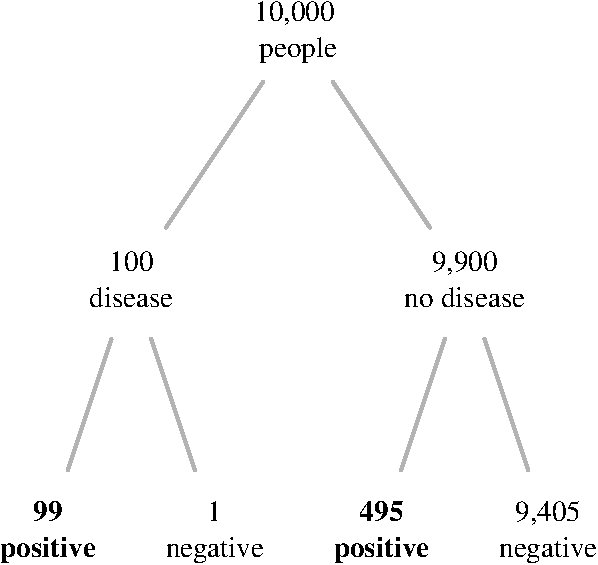
\includegraphics[width=0.8\linewidth]{03-false-positives_files/figure-latex/freq-tree-test-1}

\}

\textbackslash caption\{Out of the 594 people who test positive (shown in bold font), 99 (\textasciitilde17\%) have the disease. \}\label{fig:freq-tree-test}
\textbackslash end\{figure\}

If a randomly selected individual from this population tests positive, then it is highly likely that they do not have the disease. A positive result for this test is a terrible indicator of whether someone has the disease. This result is shocking at first. It is in stark contrast to the confidence provided by negative tests. Why?

The answer lies in the very low \textbf{base rate} of the disease. This is the same as the risk of having the disease for people within the population, which we stated as 1\%. The test has very high sensitivity and so it was able to detect almost all of the true positives. The issue was that it tested so many people who didn't have the disease, which led to many false positives. Due to the \textbf{base rate} being so low, the number of true positives (99) was much smaller (relatively) than the number of false positives (495). This meant that the positive results largely consisted of false positives.

This example outlines some statistical concepts that can lead to great insight when considering binary diagnostics. It also highlights the importance of considering a base rate. There is another statistic which can shine more light on the information that the test results have given us about the probability of disease, known as the likelihood ratio. We will revisit this example with this statistic in Chapter {[}\ldots{]}.

{[}add in an example where the base rate or the test accuracy could be changed by the user{]}

{[}add in real example using rates from home-testing coronavirus tests{]}

\hypertarget{example-doping}{%
\section{Example: doping}\label{example-doping}}

The following example has been adapted from (insert Primer citation).

It's easy to get confused with the technical terms in diagnostic tests and how they relate to the question we are interested in. Table \ref{tab:test-table} and Figure \ref{fig:freq-tree-test} present this information in a format which is easier to understand and base decisions on. However, it is often not presented this way in practice and so must first be `translated' from the raw numerical information.

\begin{quote}
A test designed to detect athletes who are doping is claimed to be `95\% accurate'. If an athlete is doping then the test returns positive 95\% of the time, and if the athlete is not doping then the test returns negative 95\% of the time. It is speculated that around 1 in every 50 athletes dope. An athlete tests positive for doping using this test during a random drugs screening. How likely is it that they are really doping?
\end{quote}

The answer is around 28\%, pause for a moment and see whether that answer comes to you from reading the above text. After reflecting on the text, continue through the example below, where we present this same information in a more familiar format.

We can convert some of the verbal information into our technical definitions. Sentence 2 states that the sensitivity and specificity are both 95\%, although those words aren't explicitly used. The base rate for doping is given as approximately 2\%.

We haven't been given a relevant population size to use natural frequencies to describe these rates, but we can imagine one in order to aid our understanding. Since we are going to use a hypothetical population of athletes, we will have to talk in terms of what we would expect from such a population, and not in terms of what we actually observe.

Assume, for clarity, that we have a relevant population of 10,000 athletes. Using the base rate, we expect 200 (2\%) of these to be doping and 9,800 (98\%) not to be doping. The sensitivity tells us that out of the expected 200 athletes who are doping, the test is expected to return positive for 190 (95\%) of them and negative for 10 (5\%) of them. We expect 10 false negatives.

Out of the expected 9,800 athletes who are not doping, the sensitivity tells us to expect 9,310 (95\%) to test negative. We expect 490 (5\%) of these non-doping athletes to test positive; we expect 490 false positives.

We expect a total of 680 positive tests and 190 (\textasciitilde28\%) of those positive tests to be from an athlete who is doping. The answer to our original question is that given a positive test result, we expect the athlete to be doping roughly 28\% of the time. This information is presented in the expected frequency tree in Figure \ref{fig:freq-tree-doping}.

\textbackslash begin\{figure\}

\{\centering 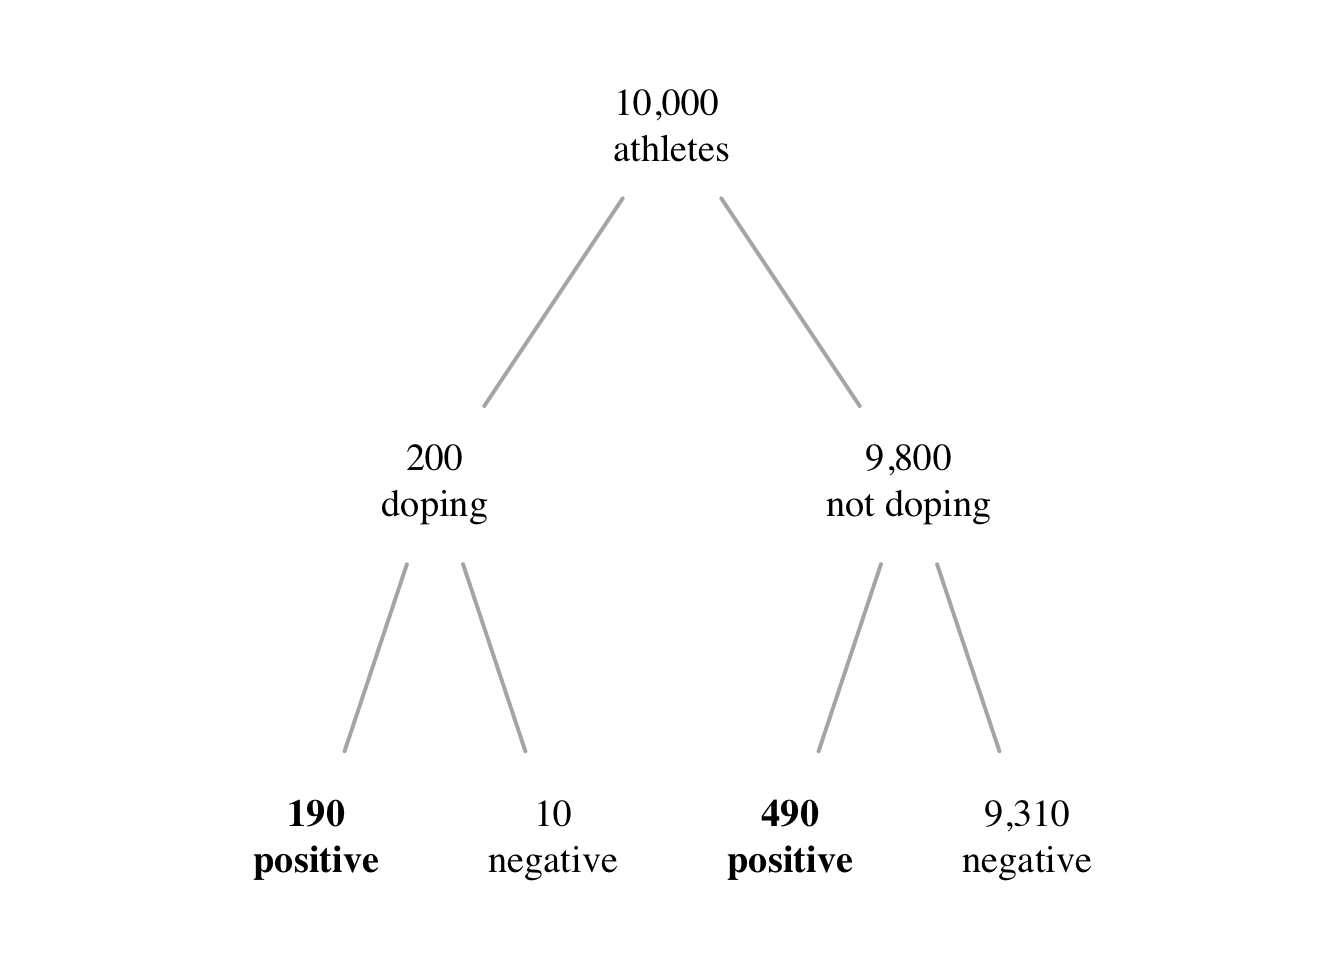
\includegraphics[width=0.8\linewidth]{03-false-positives_files/figure-latex/freq-tree-doping-1}

\}

\textbackslash caption\{Out of the 680 athletes who test positive (shown in bold font), 190 (\textasciitilde28\%) are doping. \}\label{fig:freq-tree-doping}
\textbackslash end\{figure\}

Now that we have shown that the answer to the original question is roughly 28\%, it is worth reflecting on the first sentence from the text again.

\begin{quote}
A test designed to detect athletes who are doping is claimed to be `95\% accurate'.
\end{quote}

How do you feel about this statement now? It seemed reasonable in its original context because it was the same as the sensitivity and specificity, but it seems misleading now that we know that we expect only 28\% of all positive results to be doping athletes. This is because \textbf{accuracy} is itself a technical term, and is defined by a combination of the sensitivity, specificity and, base rate. This shows how the common meaning of a word can differ from its meaning in a specific technical context, and this can lead to confusion.

This example has demonstrated that trying to answer practical questions (is an athlete doping or not based on test results) using performance information about a binary test (or other uncertain binary outcome) can be harder depending on how that information is introduced.

It hopefully also showed that clarity can be acheived by first extracting true/false positive/negative statistics from the testing context and then translating that into natural frequencies from an assumed population size. This process is not uncommon in practice as testing metrics are rarely provided in a less technical format. Presenting this information in an expected frequency tree can then provide further insight. We will revisit this example when introducing the likelihood ratio in Chapter {[}\ldots{]}.

\hypertarget{example-glass-analysis}{%
\section{Example: glass analysis}\label{example-glass-analysis}}

{[}open science data set and classification algorithm, this could be interactive where the user changes a model parameter to view the change in false positives/negatives.

We can leave this until the end of the book as a case study, combining multiple concepts from this book.{]}

\hypertarget{more-information}{%
\section{More information}\label{more-information}}

\hypertarget{exercises}{%
\section{Exercises}\label{exercises}}

\hypertarget{final-words}{%
\chapter{Final Words}\label{final-words}}

This will be a nie summary.

  \bibliography{book.bib,packages.bib,stats-book.bib}

\end{document}
